\documentclass[]{upb_cs_thesis} % include german inside brackets for a German thesis


% load your own packages and user-defined commands
\usepackage{amsmath, amssymb, amsfonts}% mathematical symbols and the like
\usepackage{amsthm}% definitions, theorems, etc.
\usepackage[colorinlistoftodos]{todonotes}% marking open todos in text/on margins
\usepackage{subfig}% multi-part figures with separate captions per part
\usepackage{url}% render URLs correctly and make them clickable through the hyperref package
\usepackage{longtable}% tables that span multiple pages
\usepackage{booktabs}% tables that actually look good
\usepackage[nolist]{acronym}% consistently use acronyms
\usepackage{caption}
\usepackage{graphicx}
%%%%%%%%%
% Some commands for setting up theorem environments as provided by package 
% amsthm --- language sensitive
%%%%%%%%%
\theoremstyle{plain}
\newtheorem{definition}{Definition}[chapter]
\newtheorem{lemma}[definition]{Lemma}
\ifgerman
	\newtheorem{theorem}[definition]{Satz}
	\newtheorem{corollary}[definition]{Korollar}
	\newtheorem{example}[definition]{Beispiel}
\else
	\newtheorem{theorem}[definition]{Theorem}
	\newtheorem{corollary}[definition]{Corollary}
	\newtheorem{example}[definition]{Example}
\fi


%%%%%%%%%
% Your commands should go here...
%%%%%%%%%
\newcommand*{\eg}{e.\,g.}
\newcommand*{\ie}{i.\,e.}
\newcommand*{\cf}{c.\,f.}
\newcommand*{\etal}{et~al.}

\newcommand{\code}[1]{\texttt{#1}\xspace}

\newacro{template}[UPB-CS-TT]{Paderborn University Computer Science thesis template}

\DeclareMathOperator{\testop}{top}





% set up some resources (graphics and bibliography)
\graphicspath{{figures/}}


%%%%%%%%%
% your thesis title, name, advisor, etc. go here;
%%%%%%%%%
\title{Technology Review}
\author {  
		\large	Arkajit Dhar\\
		\large	Ashwin Prasad Shivarpatna Venkatesh\\
		\large	Bhargavi Mohan\\
		\large	Deeksha Mysore Ramesh\\
		\large	Harshitha Pandithanahalli Somashekaraiah\\
		\large	Sanket Kumar Gupta\\
		\large	Suheel Shrirangapura Nazeersab\\
		 \large Vivek Jaganath\\~
		}
\thesistype{Technology Review}

\supervisor{ \Large \vspace*{2mm} Prof. Dr. Holger Karl  | \hspace{2mm} Sevil Dräxler  | \hspace{2mm} Hadi Razzaghi Kouchaksaraei \centering}
\submissiondate{\today{}}


% here your thesis really starts
\begin{document}
	
	% start with the titleage, the formalities, and then the abstract
	% This file defines the title page of your thesis. You typically do not need to
% edit it. It is language sensitive and prints arguments passed to commands
% \author, \title, \thesistype, \degree, \researchgroup, \supervisor and
% \submissiondate, where required.

\begin{titlepage}	
	\begin{center}
		\begin{minipage}{135mm}
			\centering
			\hbadness=10000
			
\includegraphics[height=35mm]{figures/uni-logo}			
			\textsf{
				\hspace*{8mm} 
				\Large Department of Computer Science\\
				\hspace*{8mm} Computer Networks Research Group \\
			}		
		\end{minipage}\\[40pt]
		
		
		

		{\Huge\textbf{\thetitle{}}}

	\begin{minipage}{3000mm}
	\hspace*{-1.3cm} 
	\includegraphics[height=30mm]{figures/CuK-Logo2_rot}
\end{minipage}\\[10pt]

\begin{minipage}{3000mm}
	\hspace*{-1cm} 
	
\includegraphics[height=13.5mm]{figures/subtitle}
\end{minipage}\\[10pt]

		\huge \centering \textbf{Authors:} \vspace{4mm}
	
		{\huge \textsc{\theauthor{}}}

		\ \textbf{Supervisors:}\vspace{3mm}\\ 
		
		{\huge \textsc \thesupervisor{}}\\[30pt]

		Paderborn, \thesubmissiondate{}
	\end{center}
\end{titlepage}


 % prints the title page
	%% This is the legal statement
%  - that your thesis is a work of your own,
%  - that you have not used any source other than the ones you mention, 
%  - that you genuinely created your theses to achieve the desired academic
%    degree, and have not presented it to another examination board; and
%  - that you have clearly marked all concepts and ideas that you have adopted
%    from other works.
\chapter*{Erklärung}
	\thispagestyle{empty}
	Ich versichere, dass ich die Arbeit ohne fremde Hilfe und ohne
	Benutzung anderer als der angegebenen Quellen angefertigt habe und dass
	die Arbeit in gleicher oder ähnlicher Form noch keiner anderen
	Prüfungsbehörde vorgelegen hat und von dieser als Teil einer
	Prüfungsleistung angenommen worden ist. Alle Ausführungen, die wörtlich
	oder sinngemäß übernommen worden sind, sind als solche
	gekennzeichnet.\\
	\vspace{27pt}

	\begin{center}
		\begin{tabular}{l p{0.1\textwidth} r}
			\cline{1-1} \cline{3-3}
			\begin{minipage}[t]{0.4\textwidth}
				\centering
				Ort, Datum
			\end{minipage}
			&&  
			\begin{minipage}[t]{0.4\textwidth}
				\centering
				Unterschrift
			\end{minipage}
	\end{tabular}
\end{center}

 % prints the statement that you worked on your own and did not commit plagiarism
	%\cleardoublepage
%	\vspace*{\fill}
%	\begin{abstract}
	%	\input{abstract}
%	\end{abstract}
%	\acresetall
%	\vspace*{\fill}
%	\emptypage
	
	\tableofcontents % prints the table of contents
	
	
	%%%%%%%%%
	% the contents of your thesis go into file body.tex
	%%%%%%%%%
	\listoffigures

\listoftables

\chapter{Motivation}
\label{ch:Motivation}

\section{Motivation}

The rapid growth of mobile data services driven by mobile internet has led to a substantial challenge of high availability , low latency, high bit rate and performances in networks. The recent development of Network Function Virtualization (NFV) and Software Defined Networks (SDN) has emerged as a key enabler for 5g networks. 
There has been a paradigm shift in networking with the recent developments in Network Virtualization technology. NFV involves decoupling of the hardware components from the software components of a network function. NFVs require a central management and orchestrations (MANO) framework  in order to fully deliver end to end services of an application. There are multiple open source as well as industrial implementation of a  MANO framework in the market. 

End-to-end network service delivery with high availability, scalability and low latency requires chaining of the Network Functions across different Internet Service Providers (ISPs) which in turn have their own MANO frameworks. In order to seamlessly create a network service by utilizing the Virtual Network Funtions (VNF) within each of the MANO frameworks, a common ground needs to be setup based on which the VNFs could be optimally linked to create a virtual network service.


\section{Problem Description}

European Telecommunications Standards Institute (ETSI) defines the reference architecture for a MANO framework. Each network service is composed of multiple network functions virtually linked and orchestrated by a MANO framework. The network services require a descriptor which contains the details of all the VNFs, virtual links, forwarding graph of VNFs. Each of the VNFs contain its own descriptors and the number of virtual machines it requires. Different MANO frameworks have its own descriptor schemata pertaining to the standard defined by ETSI. This framework specific Network Service Descriptor (NSD) hinders the orchestration and management of NFVs between different MANO frameworks. Our project aims at tackling this problem by implementing a method to translate and split the NFVs from different MANO frameworks in order to create a framework independent network service chain.




\chapter{Goals and Use Cases}
\label{ch:Goals and Use Cases}

In this chapter, the intended goals of the project and some use cases are being discussed.

\section{Goals}

The goal of the project is to develop a software suite which facilitates inter-operability between MANO frameworks, thereby enabling the management of a network service across a multi-vendor environment. To achieve this, the software suite is divided into 3 individual work packages (WPs), which are initially developed in parallel and are merged later. In the following sections, the individual goals of these work packages are explained in detail.

\subsection{Service Descriptor Translator (SDT)}

In this work package, a translator engine for a NSD is implemented. The Network Function Virtualization Orchestrator (NFVO) is the main orchestration unit of a MANO framework that manages the lifecycle of a network service. One of the main functions of a NFVO is registering a network service, by on-boarding it's NSD to the network service catalog. In a scenario where a network service is to be deployed among two different MANO
frameworks, having their own respective NSD schema, SDT engine would help in translating a NSD schema from one MANO framework to the other framework. 
\subsection{Service Descriptor Splitter (SDS)}

In the production environment, a network service is deployed over a vast geographical region spanning multiple domains. In such scenarios, there is a need to split a network service into smaller network services and deploy it over multiple domains. In this work package, a Service Descriptor Splitter (SDS) is implemented which splits the NSD of a network service. SDS takes NSD as an input that contains all the information elements which can be extracted to generate separate NSDs. In the proposed approach, the service graph is extracted from the input NSD and is split into subgraphs that result in a separate NSD which includes a set of elements such as VNFs, Virtual Links (VLs), forwarding graphs of VNFs etc, according to the specific MANO framework.

\subsection{MANO Adaptor (MA)}

A key component of a MANO framework is Virtualized Infrastructure Manager (VIM),  which helps in assigning the hardware resources to virtual resources. The MANO framework has specific adaptors to communicate with their respective VIMs. For instance, Sonata  (\ref{SecSONATA}) MANO framework has adaptors for OpenStack (\ref{SecOpenStack}) and Kubernetes (\ref{SecKubernetes}). However, when there is a spike in the service request beyond the capabilities of a single MANO instance, multiple MANO instances should be instantiated to balance the load. The goal of this work package is to build an adaptor that facilitates interaction between different instances of MANO frameworks, thereby exposing the underlying MANO framework's interfaces and enabling monitoring of the underlying service states.

Apart from the implementation of MA, the plan is to investigate MANO scalability challenges 


\section{Use Cases}

\subsection{Cross-MANO Framework Interaction}
The MANO frameworks used by every network service provider varies from one another. The software suite with the help of SDT and SDS enables the deployment of network services across different frameworks.

For instance: Consider two network service Operators using different MANO frameworks. One of them uses Sonata framework \cite{draxler2017sonata} and another operator uses OSM framework \cite{ersue2013etsi}. These frameworks have different NSD schemata(refer \ref{SecSONATA} and \ref{SecOSM}). NSD schemata contain VNFs, virtual links, and VNF forwarding graphs and also describes the deployment of a network service. By using a translator and splitter, these NSD schemata can be translated and split into a framework-specific schema. With this, operators can deploy and manage network services across different MANO implementations.

\subsection{Hierarchical Orchestration}
By using MA, dynamic instantiation of multiple MANO instances and inter-operability between different MANO frameworks can be achieved. The operator will be able to handle the resources in an efficient manner, as one MANO framework can manage a limited number of service requests, operators can explore options to include additional MANO instances under the existing MANO instance to mitigate the traffic load on a single instance. The resources can be provisioned based on the number of requests. This helps the operator in extending their profitability.

\textbf{Actors} : The Network Service Providers who would use features of SCrAMbLE.

\begin{figure} [h]
	\centering
	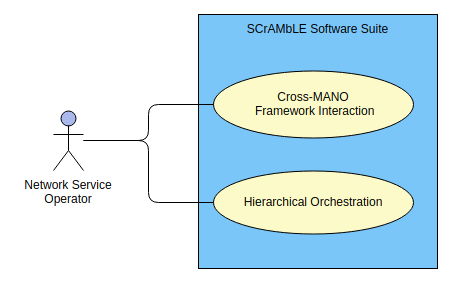
\includegraphics[width=0.9\linewidth]{figures/use-case}
	\caption{Use Case Diagram}
	\label{fig:use-case}
\end{figure}










\chapter{Technologies}
\label{ch:Technologies}
\section{MANO Frameworks}
\paragraph{}
In this section, a few MANO frameworks and their NSD schemata are listed(list of a few parameters and their description). Among several frameworks, the plan is to select a few and set them up locally, deploy network services and support them in the project. This list is subjected to future additions or removals.
\subsection{OpenBaton}
\paragraph{}
Open Baton is an open source implementation of ETSI MANO specification. It's main objective is to develop an extensible and customizable framework capable of orchestrating network services from different domains\cite{openBaton}. Following table lists the important parameters of NSD\cite{openBatonSchemaDocumentation}. 
    \begin{table}[h]
        \centering
        \begin{tabular}{ |p{4cm}|p{10cm}|}
            \hline
            \textbf{Parameter} & \textbf{Description} \\
            \hline
             
             Name & The name of the network service \\
             \hline
             Vendor & The vendor or provider of the network service \\
             \hline
             Version & The version of the network service (can be any string) \\
             \hline
             vnfd & The list of VNFs composing the network service (see Virtual Network Function Descriptor for more details) \\
             \hline
             Vld & The list of Virtual Links that are referenced by the VNF Descriptors in order to define network connectivity \\
             \hline
             Vnf\_dependency & The list of dependencies between VNFs\\
             \hline
        \end{tabular}
        \caption{Open Baton NSD parameters}
        \label{tab:OpenBatonSchema}
    \end{table}
\subsection{SONATA}
\label{SecSONATA}
\paragraph{}
SONATA is one of the NSO research projects which targets two crucial technological challenges in the foreseeable future of 5G networks as follows\cite{SONATA}.
\begin{itemize}
    \item Flexible programmability
    \item Deployment optimization of software networks for complex services /applications.
\end{itemize}
SONATA complies with the ETSI NFV-MANO reference architecture. Following tables lists the important parameters of NSD \cite{SONATASchemaDocumentation}.
\subsubsection{Network Service Descriptor Section}
    \begin{table}[h]
    \centering
    \begin{tabular}{ |p{4cm}|p{10cm}|}
        \hline
        \textbf{Parameter} & \textbf{Description} \\
        \hline
         
         Vendor & Identifies the network service uniquely across all network service vendors. \\
         \hline
         Name & Name of the network service without its version. \\
         \hline
         Version & Names the version of the NSD. \\
         \hline
         Author & It's an optional parameter. It describes the author of NSD \\
         \hline
         Description & It's an optional parameter, provides an arbitrary description of the network service. \\
         \hline
    \end{tabular}
    \caption{SONATA: Network Service Descriptor Section}
    \label{tab:SONATA_general_section}
\end{table}
\subsubsection{Network Functions Section}
    \begin{table}[h]
    \centering
    \begin{tabular}{ |p{4cm}|p{10cm}|}
        \hline
        \textbf{Parameter} & \textbf{Description} \\
        \hline
         
         network\_functions & Contains all the VNFs that are handled by the network service. \\
         \hline
         Vnf\_id & Represents a unique identifier within the scope of the NSD \\
         \hline
         Vnf\_vendor & As part of the primary key, the vendor parameter identifies the VNF Descriptor \\
         \hline
         Vnf\_name & As part of the primary key, the name parameter identifies the VNF Descriptor \\
         \hline
         Vnf\_version & As part of the primary key, the version parameter identifies the VNF Descriptor\\
         \hline
         Vnf\_description & It's an optional parameter, a human-readable description of the VNF\\
         \hline
    \end{tabular}
    \caption{SONATA: Network Functions Section}
    \label{tab:SONATA_NF_section}
 \end{table}
\subsection{TeNOR}
Developed by T-NOVA project, it's the NFV Orchestrator platform which is not only responsible for the entire lifecycle service management of NFV but also optimizing the networking and IT resources usage. Network service and VNF descriptors follow the TeNORs data model specifications that are a derived and an extended version of the ETSI NSD and VNF Descriptor data model \cite{de2018network}. Following table lists some of the parameters of the descriptors \cite{TeNorSchemaDocumentation}.
    \begin{table}[h]
        \centering
    \begin{tabular}{ |p{4cm}|p{10cm}|}
        \hline
        \textbf{Parameter} & \textbf{Description} \\
        \hline
         
         Id & Unique ID of the network service \\
         \hline
         Name & Name of the network service \\
         \hline
         Vendor & Identifies the network service uniquely across all network service vendors \\
         \hline
         Version &  Names the version of the NSD \\
         \hline
         Manifest\_file\_md5 & Exposes MD5 check-sums of the meta-data that the manifest file contains \\
         \hline
         vnfds & Array of VNF Descriptors \\
         \hline
    \end{tabular}
        \caption{TeNOR: Network Service Descriptor}
    \label{tab:TeNOR_NSD_section}
 \end{table}
\newpage
\subsection{Cloudify}
\paragraph{}
Cloudify is an open source cloud orchestration framework mainly focused on optimization of NFV Orchestration and management. It provides a TOSCA based blueprint which facilitates end-to-end lifecycle of NFV Orchestration. Cloudify follows MANO reference architecture but not entirely compliant to it\cite{de2018network}. Following are some high-level sections of the blueprint which describes the network services that are installed and configured \cite{CloudifySchemaDocumentation}.
    \begin{table}[h]
        \centering
    \begin{tabular}{ |p{4cm}|p{10cm}|}
        \hline
        \textbf{Parameter} & \textbf{Description} \\
        \hline
         
         type & The node-type of this node template \\
         \hline
         properties &   The properties of the node template, matching its node type properties schema \\
         \hline
         instances &    Instances configuration(deprecated replaced with capabilities and scalable) \\
         \hline
         interfaces  & Used for mapping plugins to interface operation, or for specifying inputs for already-mapped node type operations \\
         \hline
         relationships &    Used for specifying the relationships that this node template has with other node templates \\
         \hline
         capabilities & Used for specifying the node template capabilities. (Supported since: cloudify\_dsl\_1\_3) Only the scalable capability is supported\\
         \hline
    \end{tabular}
    \caption{Cloudify: Node Template}
    \label{tab:Cloudify_node_template}
 \end{table}
\subsection{Open Source MANO(OSM)}
\label{SecOSM}
\paragraph{}
OSM is an open source management and orchestration stack in compliant with ETSI NFV information models. OSM architecture splits between resource orchestrators and service orchestrators \cite{de2018network}. Table \ref{tab:OSM_nsd} lists the parameters of NSD schema. \cite{OSMSchemaDocumentation}
    \begin{table}[h]
        \centering
    \begin{tabular}{ |p{4cm}|p{10cm}|}
        \hline
        \textbf{Parameter} & \textbf{Description} \\
        \hline
         
         id &   Identifier for the NSD \\
         \hline
         name & NSD name \\
         \hline
         Short-name &   Short name which appears on the UI \\
         \hline
         vendor &   Vendor of the NSD \\
         \hline
         logo & File path for the vendor specific logo. For example, icons/mylogo.png. The logo should be a part of the network service. \\
         \hline
         description &  Description of the NSD \\
         \hline
         version &  Version of the NSD \\
         \hline
    \end{tabular}
        \caption{OSM: Network Service Descriptor}
    \label{tab:OSM_nsd}
 \end{table}



\newpage
\section{Virtualized Infrastructure Manager (VIM)}
VIM is one of the three functional blocks specified in the Network Functions Virtualization Management and Orchestration (NFV-MANO) architecture. VIM is responsible for controlling and managing the NFV Infrastructure (NFVI), by provisioning and optimizing the allocation of physical resources to the virtual resources in the NFVI. Performance and error monitoring is also a key role of the VIM. Popular VIMs are discussed in the following sections.
\subsection{OpenStack}
\label{SecOpenStack}
\paragraph{}
OpenStack\footnote{https://www.openstack.org/} is a community-driven open source cloud resource management platform. Compute, storage, and networking resources in a data center can be provisioned using Application Program Interfaces (APIs) or web dashboard provided by OpenStack component, for instance, NOVA is a component which can provide access to compute resources, such as virtual machines and containers. Network management is enabled by NEUTRON component which handles the creation and management of a virtual networking infrastructure like switches and routers. SWIFT component provides a storage system. By making use of many such components, OpenStack can deliver complex services by utilizing an underlying pool of resources.
\subsection{Amazon Web Services (AWS)}
\paragraph{}
AWS\footnote{https://aws.amazon.com/} is a cloud computing platform, It offers (1) Infrastructure as a Service (IaaS) -- provides resources that can be utilized for custom applications (2) Platform as a Service (PaaS) -- provides services such as database and email which can be used as individual components for building complex applications (3) Software as a Service (SaaS) -- provides user applications with customization and administrative capabilities that are ready to use. AWS is specially preferred by small companies for the flexibility and ease of use of it's cloud infrastructure.
\subsection{Kubernetes}
\label{SecKubernetes}
\paragraph{}
Kubernetes\footnote{https://kubernetes.io/} (K8s) is an open-source platform for automation and management of containerized services, it manages computing, networking, and storage infrastructure. Kubernetes was initially developed by Google and now under Cloud Native Computing Foundation. Kubernetes Architecture consists of (1) Master server components -- it is the control plane of the cluster and act as the gateway for  administrators (2) Node Server Components -- servers which are performing work by using containers that are called nodes, they communicate with the master component for instructions to run the workload assigned to them. Kubernetes provides comprehensive APIs which are used to communicate between the components and with the external user.


\chapter{Related Work}
\label{ch:Related Work}

\paragraph{}
In this chapter we discuss the relevant research efforts that can be used to achieve our goals. First we discuss the standards and specifications for orchestration and management of NFV in the section \ref{standSpecs}. The fundamental aspect of a service deployment is the Network Service Descriptor (NSD), in the section \ref{serviceDescription} we discuss the trends and options of NSDs. In section \ref{interopmano}, we discuss research papers that try to mitigate the interoperability challanges between different MANO frameworks. Section \ref{manoscale} will be a brief account on the MANO scalability problem.\\

As this is our initial project proposal, the state-of-the-art could change as we progress and we will update our approach accordingly.


\section{Standards and Specifications}
\label{standSpecs}

\cite{rotsos_network_2017}
\cite{de_sousa_network_2018}
\cite{yong_li_software-defined_2015}

\section{Service Description}
\label{serviceDescription}

\cite{garay_service_2016}

\section{MANO Interoperability}
\label{interopmano}


\section{Hierarchical Orchestration }
\label{manoscale}

\paragraph{}
MANO framework face significant scalability challenges in large scale deployments, the amount of infrastructure a single instance of MANO framework can manage is limited. Abu-Lebdeh et al. \cite{abu-lebdeh_nfv_2017} explores the effects of placement of MANO on the system performance and scalability and conclude by suggesting hierarchical orchestration architecture to optimize them, they formally define the scalability problem as an integer linear programming and propose a two-step placement algorithm. We also intend to answer the MANO scalability challenges, by exploring the optimal number of MANO deployments in a system, the optimal hierarchical level and how to manage the state of such a system dynamically.


\chapter{Project Time Plan}
\label{ch:Project Time Plan}

In this section, the time plan for the project is discussed, which provides an overview of different tasks and what the team achieves for the course of one year. The intention of this timeline is to provide a rough idea over the tasks and their duration. The actual plan will be decided and defined as the project proceeds further. For better understanding, the main tasks of the project are divided as shown in the table below.

\begin{table} [h]
\centering
	\begin{tabular}{|c|l|c|c|}
	\hline
		Sr.No. & Tasks & Start & End\\
		\hline
		1 &	Project organization & 11.10.2018 &	10.11.2018\\
		\hline
		2 &	Preparation and Presentation of mini seminar & 11.10.2018 &	19.11.2018\\
		\hline
		3 &	Developing Project Plan & 20.11.2018 & 06.12.2018\\
		\hline
		4 &	Reviewing Technologies & 20.11.2018 & 20.12.2018\\
		\hline
		5 &	Designing Architecture &	06.12.2018 & 31.01.2019\\
		\hline
		6 & Implementation and Deployment &	07.02.2019 & 30.08.2019\\
		\hline
		7 & Presentation &	01.09.2019 & 20.09.2019\\
		\hline
	\end{tabular}
\caption{List of all tasks in the time plan}
\end{table}

The following list further defines the goals of each task: 
\begin{enumerate}
	\item \textbf{Project organization:}
	To establish communication between team members to understand each other, in terms of their skills set and expertise. Also, decide upon tools for project management, task management, version control and a platform for all further communications. As an outcome, we have decided to use Gitlab for project, task management and for version control, Texstudio for documentation and Slack for internal communication.
	\item \textbf{Preparation and Presentation of mini seminar:}
	To get an overview of various technologies and subjects that is required for the project. Select one of the subjects, research the subject in depth and present the concepts that are relevant to the project, to the team.
	\item \textbf{Developing project plan:}
	To combine all the subjects presented by each team member and make a basic sketch of what to achieve, how to achieve and by when to achieve it. For the project group, the document is a valuable reference to get an overview of the problem, related technologies and required sub-tasks. 
	\item \textbf{Reviewing technologies:}
	To list all the technologies that are relevant to the project, review pros and cons of each technology and to decide upon technologies to be used in the project.
	\item \textbf{Designing architecture:}
 The aim here is to discuss, design and document the base for implementation. 	We have divided the project group into sub-groups who will decide on technologies and methods for implementation. The divided sub-groups is as follows.
 
\begin{table} [h]
	\centering
	\begin{tabular}{|c|c|c|}
		\hline
		WP1 & WP2 & WP3 \\
		\hline
		Arkajit & Sanket & Ashwin \\
		\hline
		Vivek &	Harshitha & Bhargavi \\
		\hline
		Suheel &  & Deeksha \\
		\hline
	\end{tabular}
	\caption{Details of sub-groups}
\end{table}
	
	This phase is one of the most crucial phases in the project group, as it is a core foundation to the project.
	\item \textbf{Implementation and Deployment:}
	 Each sub-group working independently on their respective work packages and discuss the updates with team on weekly basis. Integrate and test the end product by benchmarking and by defining various scenarios where the product can be tested and to produce a stable product by the end of the implementation phase. This requires maximum efforts and time, as various versions/prototypes will be developed until a satisfying and stable end product is obtained. Implementation can be done in following stages.
	
		\begin{itemize}
		\item\textbf{Initial Development}: sub-groups working independently on respected packages.
		\item\textbf{Unit Test}: Conduct testing on each of the packages developed
		\item\textbf{Integration}: Integrate work of all the sub-groups.
		\item\textbf{Final Testing}: Use benchmarking and test the final product. 	
	\end{itemize}


	\item \textbf{Presentation:}
	After implementing the system, it is presented to the supervisors. This is achieved by presenting in document or pictorially the end results obtained by the produced developed. Present the learnings, challenges and benefits from the end product produced. 
	\end{enumerate}

\begin{figure}[h]
\centering
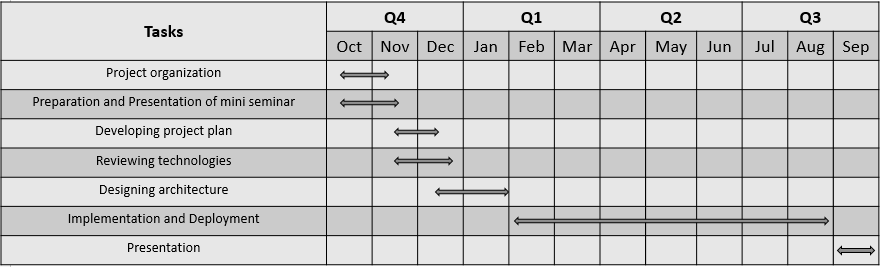
\includegraphics[scale=.6]{timeplan}
\caption{A gantt diagram visualizing the time plan.}
\end{figure}
The sequence of the tasks is visualized in the above diagram. Though the timeline mentioned is fixed and can change during the course of various phases of the project, this is to constantly remind the deadlines and to foresee further responsibilities and milestones to be achieved. 


	

\chapter{Conclusion}
\label{ch:Conclusion}
As discussed previously, there are many challenges to overcome and milestones to be achieved.
At the end, the goal is to build an end product, i.e. OSM adaptor, NSD Splitter and NSD translator but 
an in-depth knowledge on how to achieve it is needed. The next step is to use this document as a base and start reviewing all the technologies and decide upon which ones to use. Design and documention of the architecture which is the foundation to implement the project will begin.
Also in order to be efficient, The project group is divided into sub-groups, to work independently on various topics. Every week the progress of each sub-group is reviewed toshare knowledge and findings to rest of the team. Ultimately, collaborate all the results of the sub-groups to produce a stable end product. 




	
	% include the bibliography, and add it as a chapter the table of contents
	\newpage
	\addcontentsline{toc}{chapter}{Bibliography}
	\bibliographystyle{alpha}
	\bibliography{literature}
	
	
	%%%%%%%%%
	% the appendices of your thesis go into file appendix.tex
	%%%%%%%%%

	\end{document}
